\documentclass[notitlepage]{article}
\usepackage{graphicx}
\usepackage{bmpsize}
\usepackage{color}
\usepackage{courier}
\usepackage{listings}
\usepackage{times}
\usepackage[T1]{fontenc}
\usepackage{textcomp}
\usepackage{fullpage}
\usepackage{hhline}
\usepackage{tabular x}
\usepackage{mdframed}
\usepackage{enumerate}
\usepackage{titlesec}
\usepackage{hyperref}
\usepackage[clock]{ifsym}

\lstset{language=VHDL}
\lstset{basicstyle=\normalsize\ttfamily,breaklines=true}
\graphicspath{ {img/} }
\newcommand{\sectionbreak}{\clearpage}
\newcommand{\infosign}{\fontencoding{U}\fontfamily{futs}\huge\selectfont\char 116\relax}
\newcommand{\warningsign}{\fontencoding{U}\fontfamily{futs}\Large\selectfont\char 66\relax}
\newcommand{\dangersign}{\fontencoding{U}\fontfamily{futs}\huge\selectfont\char 76\relax}
\newmdenv[linecolor=black,skipabove=\topsep,skipbelow=\topsep,
leftmargin=0pt,rightmargin=0pt,
innerleftmargin=5pt,innerrightmargin=5pt]{infobox}
\makeatletter
\newcommand*{\toccontents}{\@starttoc{toc}}
\makeatother

\begin{document}

\title{\huge{\texttt{ratload}\\ Installation and Use}}
\author{
  Jacob Hladky\\
  California Polytechnic State University\\
  San Luis Obispo, CA\\
  \texttt{jhladky@calpoly.edu}
}
\date{\today}
\maketitle

\toccontents

\pagenumbering{arabic}

\section{Introduction}
\texttt{Ratload} is a system for loading new RAT assembly programs on to the RAT CPU without the need for resynthesis.\\\\
The system consists of two components: a computer program and a set of VHDL modules. This guide will detail how to install, use, and --- if necessary --- troubleshoot both. This guide is for Windows users, but \texttt{ratload} can also be run on GNU/Linux and OS X. Instructions for those platforms are in a separate document, called ``linux\_and\_osx.pdf''.

\subsection{Requirements}
If you have a Nexys 2 board --- You will need a serial cable. If your computer does not have a serial port, then you will need a USB-to-serial adapter. Here's an example: \url{http://amzn.com/B00065H0QQ}. Any adapter will do as long as you have the right drivers for it.\\
If you have a Nexys 3 board --- No serial cable is required, but you will need another micro-USB cable.\\\\
Do not integrate ratload into your RAT CPU until all the major components of the CPU are in place, and you have a good understanding of how they fit together. Understanding how the RAT architecture handles I/O and interrupts will make integration much easier.

\subsection{Project Manifest}
The following is a general overview of the files in the system.
\begin{itemize}
\item \texttt{README.pdf} This guide.
\item \texttt{linux\_and\_osx.pdf} Instructions for using ratload on GNU/Linux and OS X platforms.
\item \texttt{new\_rat\_wrapper/} VHDL files necessary to integrate the new rat\_wrapper.
\item \texttt{new\_prog\_rom/} VHDL files necessary to integrate the new prog\_rom.
\item \texttt{testing/} Files for testing the operation of the new system.
\item \texttt{ratload\_v{\textless}version\textgreater} The ratload program.
\end{itemize}

\subsection{Bug Reporting}
All programs have bugs. \texttt{ratload} is beta software and is no exception. If you encounter a bug in the ratload program, please contact the author. It is also possible that you find a bug in the project VHDL modules. If you do please verify the bug via simulation and report it immediately so it can be fixed.\\\\
Since you are writing the mechanics of the CPU itself, it is possible for very odd bugs to happen, and for those bugs to interact with \texttt{ratload} in bizarre ways\ldots Please note that \texttt{ratload} has been thoroughly tested and is free of any major bugs.

\subsection{Project Information}
If you have any questions about the project itself, or suggestions for improvement for this guide, please contact the author at jhladky@calpoly.edu. This project licensed under the MIT license and the complete source code --- including the \LaTeX ~source for this guide --- is available at \url{http://www.github.com/jhladky/ratload}. Ratload system releases are available at \url{http://homecrest.hladky.me/ratload/}.\\\\
This project uses a UART module authored by Peter A. Bennett and released under the LGPL. The source for that module is available at \url{https://github.com/pabennett/uart}.

\subsection{Changelog}
Version 1 03/02/15
\begin{itemize}
  \item Initial project release.
\end{itemize}
Version 2 03/04/15
\begin{itemize}
\item Switched to using a new UART.
\item Fixed a bug in the UART wrapper where the interrupt wasn't being asserted for more than one clock tick. In CPUs that only checked for the interrupt flag in one clock cycle, the interrupt wouldn't be detected.
\item Renamed ``serial\_test'' directory to ``testing''.
\item Added reference bit file to ``testing'' directory.
\item Clarified and improved some of the installation instructions, and added instructions about using the reference bit file to the troubleshooting section. Added a section about interrupts.
\end{itemize}
Version 3 03/05/15
\begin{itemize}
\item Fixed a bug in the ratload program where serial device names would be concatenated together.
\item Added an instruction in Section 3 telling users to remove any previous prog roms, and fixed typos in Secs 2.1 and 2.2.
\item Renamed ``Contact'' section to ``Project Information''. Added credit for UART module.
\end{itemize}

\section{Adding the New RAT Wrapper}
\texttt{Ratload} requires a UART to communicate with the host computer, which is provided as part of a new RAT wrapper module, which will replace your current wrapper. The new RAT wrapper provides access to the LEDs, and the buttons, and the switches, and the 7-segment display. If you want to add any more I/O devices, such as the VGA driver buffer, you will need to add them manually.

\begin{infobox}
  {\infosign} UART stands for ``Universal Asynchronous Receiver-Transmitter'', which you may recognize as another name for a serial port. The UART can be used outside of the \texttt{ratload} system as well. If you would like more info about using the UART in your final project, contact the author.
\end{infobox}

\subsection{Integration with RAT CPU}

\begin {enumerate}

\item Make a backup copy of your CPU right now! You are about to make some big changes to your project and you'll want something to fall back on in case something goes wrong.

\item Remove your RAT wrapper VHDL module, making your RAT CPU module the top-level module. Also remove your RAT wrapper ucf file.

\begin{infobox}
  {\warningsign} Double check you have backed up your RAT project! Otherwise you could lose everything!
\end{infobox}

\item Navigate to the \texttt{ratload} project directory (where this README is located), and then to the ``new\_rat\_wrapper'' directory. If you have a Nexys 2 board, \underline{delete} the ``rat\_wrapper\_nexys3.ucf'' file and rename the ``rat\_wrapper\_nexys2.ucf'' file to ``rat\_wrapper.ucf''. If you have a Nexys 3 board, do the opposite.

\item Go to \textbf{Project \textgreater Add Copy of Source}. Select all the files in the ``new\_rat\_wrapper'' directory and click \textbf{Open}. Another dialog box will pop up confirming you want to add these files. Click \textbf{OK} to confirm.

\item Go to \textbf{Project \textgreater Design Goals \& Strategies}. Change the \textbf{Design Goal} to \textbf{Timing Performance}. Click \textbf{Apply} and then \textbf{OK}.

\item Go to \textbf{Project \textgreater Cleanup Project Files\ldots}. Click \textbf{OK}. This will ``refresh'' your project. Sometimes synthesis can fail for what seems like no reason, and this step is intended as a prevention of that. If you experience another such failure, repeat this step.

\item That is all that's necessary to add the new RAT wrapper. However the signal names of your \textbf{RAT CPU module} may differ from those declared in the RAT wrapper. Change the signal names in the new RAT wrapper as necessary and make sure you can generate a bit file.
\end{enumerate}

\subsection{Verification}
\label{sec:verification}
This section covers a quick test of the new RAT wrapper. you just integrated into your RAT CPU. If the test in this section is not 100\% successful \textbf{DO NOT CONTINUE}. Go back and double check that you have integrated the UART properly. If the UART continues not to work, see Section~\ref{sec:troubleshooting}. \texttt{Ratload} \textbf{WILL NOT WORK} unless your UART behaves exactly as expected!

\begin{enumerate}
\item Delete your current prog\_rom module from ISE by right-clicking on the file and clicking \textbf{Remove}. Then right-click again and select \textbf{Add Copy of Source}. Navigate to the ``testing'' directory and add the ``serial\_test.vhd'' file. This will replace your current prog\_rom module with the prog\_rom module in the ``serial\_test.vhd'' file.

\item Program your Nexys board with the new bit file.

\begin{infobox}
  {\infosign} The next steps involve running the ratload program. For more information about installing and running the ratload program see Section~\ref{sec:installation}.
\end{infobox}

\item Connect your serial cable between the Nexys board and the host computer. Open the ratload program and select the proper serial device from the dropdown menu. Ignore the ``Choose File...'' prompt. If you are having trouble identifying your serial device, see Section~\ref{sec:serial_id}.

\item Go to \textbf{Menu \textgreater Run Serial Test}. The program will then attempt to communicate with the Nexys board via the serial cable.

\item If the test indicates ``PASS'', proceed to the next section. Otherwise go straight to Section~\ref{sec:troubleshooting}. Do not pass Go. Do not collect \$200.
\end{enumerate}

\section{Adding the New Prog\_Rom module}
Once you have added the UART and verified that it is functioning correctly, the remaining steps are simple.
\begin{enumerate}
\item Select the prog\_rom file in your RAT CPU and right-click \textbf{Remove}.

\item Go to \textbf{Project \textgreater Add Copy of Source}. Navigate to the ``new\_prog\_rom'' directory and select all the modules within. Click \textbf{Open}. Another dialog box will pop up confirming you want to add these files. Click \textbf{OK}. If it asks you about overwriting any files, click \textbf{OK}.

\item In the architecture section of the rat\_cpu module, edit the component declaration for the prog\_rom module. Add the following line:\\
  \centerline{\texttt{TRISTATE\_IN : in STD\_LOGIC\_VECTOR(7 downto 0)}}

\item In the same file, edit the port map decaration for the prog\_rom module. Map the signal for the RAT CPU's tristate bus into to the prog\_rom module's tristate bus. The RAT CPU's ``tristate\_bus'' may be called the ``MULTI\_BUS'' in your CPU. (Regardless of its name, this is the bus that connects the ALU, the program counter, the scratch pad, and others.) That line will look similar to this:\\
  \centerline{\texttt{tristate\_in =\textgreater ~tristate\_bus\_sig(7 downto 0),}}

\item Synthesize and generate a bit file for your newly integrated system. That's it! \texttt{Ratload} should work on your CPU now. The next sections cover installing and using the ratload program.
\end{enumerate}

\section{Installation and Use of the ratload Program}
\label{sec:installation}
\subsection{Installing ratload}
Installation is really easy. The ratload program is located in the a directory called ``ratload\_v{\textless}version\textgreater'', where {\textless}version\textgreater~is replaced by whatever version the program happens to be in. Simply copy that directory to someplace useful to you. Run the program by running ``app.exe''. There is no other installation step.\\\\
If a GUI is too fancy for you then you can also use the command line version of ratload. Instructions for doing so are available in the ``linux\_and\_osx'' PDF also included in this project.

\subsection{Operational Overview}
Up until now, you've probably followed this pattern when developing your assembly language programs:
\begin{enumerate}
\item Run your assembly repeatedly in the ratsim program until it produces a prog\_rom.vhd file and seems to be bug free.
\item Add the new prog\_rom.vhd file to your project, replacing the old one.
\item Resynthesize the entire project and reprogram the bit file onto your Nexys board.
\item Repeat ad infinitum.
\end{enumerate}
The steps you have just followed to integrate the vhd files into your RAT CPU, and to install the ratload program onto your computer, will dramatically change this pattern. From now on you do not need to resynthesize your project when ratsim generates a new prog\_rom.vhd file, nor is it necessary to copy that new file into your project. In fact, \textbf{making any more changes to the prog\_rom.vhd file in your project directory will break \texttt{ratload}}.\\\\
This section contains instructions for identifying the serial device you need to use to communicate with the Nexys board, an overview of the \texttt{ratload} procedure, and instructions on using either the command-line or the graphical (Windows only) ratload program.

\subsection{Identifying your Serial Device}
\label{sec:serial_id}
How you identify your serial device will depend on what Nexys board you have as well as whether you are using a USB-serial adapter or not. Before you identify your serial device you need to make sure you have the correct drivers installed for it. This sounds a lot more complicated than it really is. Follow either of the following sections based on which Nexys board version you have to make sure you have the right drivers installed.

\subsubsection{Nexys 2}
If you have a serial port on your computer, congratulations, you are using a computer from the 20th century! Windows probably already has installed drivers to use this port, so you don't need to do anything else.\\\\
If you don't have a serial port, then you need to obtain a USB-to-serial adapter cable. The manufacturer of the cable probably provided drivers for you to install along with the cable itself. Try to google around to try to find the right driver.\\\\
Once you think you've installed the driver then you simply need to verify that the OS can see it. Go to \textbf{Start} menu and \textbf{right-click Computer}, and then click \textbf{Manage}. Look for the serial device in the \textbf{Device Manager}.

\subsubsection{Nexys 3}
If you have a serial port on your computer, it doesn't matter, you can't use it! The Nexys 3 doesn't have a physical serial port, but instead emulates one. Those drivers should have been installed when you installed the Adept software, so you're good to go.

\subsubsection{Finding the port name}
Run the graphical ratload program. The main window of the program contains a dropdown which lists your available serial devices. If you are using a USB-to-serial adapter the easiest way to be totally sure of the correct COM port number is to unplug the adapter and note the adapters listed. Then plug in the adapter and click \textbf{File > Refresh Serial Devices}. The COM port that appears in the dropdown is the COM port of the adapter.

\subsection{Ratload Procedure}
\begin{enumerate}
\item Program your Nexys board with the generated bit file.

\item Without disconnecting anything else, connect the Nexys 2 board to your computer via the serial cable. If you have a Nexys 3 board, connect the second USB cable for the UART.

\item Start the ratload program. Select the proper serial device and prog\_rom.vhd file to read.

\item The program will then communicate with the Nexys board and send the prog\_rom.vhd to your RAT CPU via the serial connection. Once the program displays a success message, the serial cable can be disconnected and the board used normally. You can treat the program running on the board like it was synthesized with the system using the previous pattern, with one exception. For more information about this exception see Section~\ref{sec:interrupts}.

\item To send a new prog\_rom.vhd file you must power cycle your Nexys board and repeat this procedure, starting with Step 1.
\end{enumerate}

\subsection{Interrupts and the ratload System}
\label{sec:interrupts}
\texttt{Ratload} uses a UART to communicate with the host computer. The UART requires an interrupt, and the RAT CPU only has one interrupt. This creates a problem if you want to add I/O devices like a mouse, that also require an interrupt. A suggested solution is to \texttt{OR} the interrupts together.\\\\
Because the UART is only active during the programming stage, it will not trigger an ISR while your program is running. A more extensible solution would be to add multiple I/O interrupts, but for our purposes this is sufficient.

\section{Troubleshooting}
\label{sec:troubleshooting}

\subsection{Checking your serial cable with the reference bit file}
The following procedure will verify that your serial adapter is working and that the ratload program is working. Loosely speaking, this section tests the ``host side'' of the system, whereas subsequent sections test the ``VHDL side'' of the system.

\begin{enumerate}
\item Program your Nexys board with the ``rat\_wrapper.bit'' file included in the ``testing'' directory.
\item Connect your serial cable between the Nexys board and your computer.
\item Follow the steps in Section~\ref{sec:verification} starting from step 4.
\end{enumerate}

\subsection{Troubleshooting the UART Module}
The easiest way to troubleshoot the UART module is to break out an actual serial console and see what it's sending to the computer. So that's what we're going to do. You will need to know what your serial device is called on your computer. To do so see Section~\ref{sec:serial_id}.
\subsubsection{Obtaining a serial console}
A good serial console for Windows is RealTerm. Download and install it from here: \url{http://www.i2cchip.com/realterm/}

\begin{figure}[ht!]
  \centering
  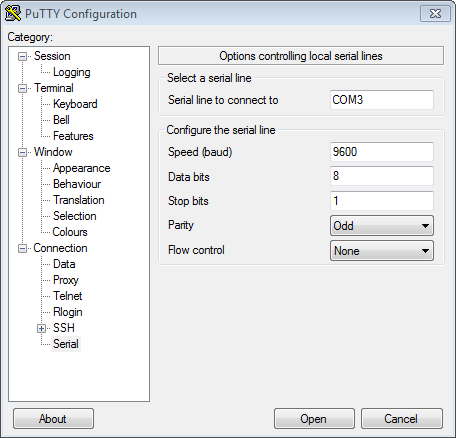
\includegraphics[width=0.75\textwidth]{fig0.png}
  \caption{The correct settings to use with RealTerm}
  \label{fig:realterm}
\end{figure}

\subsubsection{Configuring the proper serial console settings}
Run RealTerm. Click on the \textbf{Port} tab. Make your RealTerm settings look like they do in Figure~\ref{fig:realterm}. Make sure to click \textbf{Change} to apply the settings. Remember that your COM port may differ.

\subsubsection{Using the serial console to troubleshoot the UART}
Once you have your serial console up and running flash your Nexys board with your bit file that has the serial test program on it. (Make sure you've connected the Nexys board to your computer with the serial cable).\\\\
Send some data to the UART from the serial console. This is done by typing in the serial console. The behavior of the serial test program is as follows:
\begin{enumerate}
\item Get an ASCII-encoded byte from the host computer.
\item Convert that byte to binary
\item Display the byte on the LEDs on the Nexys board.
\item Re-encode the same byte to ASCII and send it back to the host computer.
\end{enumerate}
You are looking for the following behavior when interacting with the serial test program:
\begin{enumerate}
\item Send 1 ASCII-encoded byte
\item Receive that same byte back.
\end{enumerate}
If you receive two characters back, if you receive no characters back, if you receive a flood of characters back, or anything that is not that exactly what you typed, then you have integrated the RAT wrapper incorrectly.

\subsection{Troubleshooting the Ratload program}
Ratload can fail in several different ways. This section lists all possible error messages, an explanation of each, and a suggestion on how to resolve the error.

\begin{itemize}
\item ``File not found'', or similar: Ratload could not open your prog\_rom.vhd file. Perhaps it couldn't find it, or it didn't have permission.
\item ``Port not found'', or similar: Ratload could not open the serial device you specified. Perhaps you specified it incorrectly, or ratload does not have permission to access it.
\item ``Invalid prog\_rom.vhd file.'': Ratload was able to find and open the file you specified, but it couldn't parse it. Ratload expects the prog\_rom.vhd to be structured in a very specific way. Because this file is auto-generated by the ratsim program, this is not a problem. Make sure you are specifying the exact prog\_rom.vhd file that ratsim generates. If you continue to receive this error, try generating the prog\_rom.vhd file again.
\item ``Serial Configuration Failed'', or similar: Ratload was able to find and open the device you specified, but when it failed to configure it. It is possible but extremely unlikely that you have a serial device that does not support the proper settings. It is much more like that you specified a valid but incorrect device.
\item ``Handshake with Nexys board failed.'': Ratload was able to open initial communication with the Nexys board but received bad data. Get out the serial terminal and see what data the is actually being send out.
\item ``Received bad data from Nexys board.'': Ratload was able to open and parse the file you specified, and was able to open and configure the serial device you specified, but it received no or incorrect data from the Nexys board. Program the ``reference\_rat\_wrapper.bit'' file onto your Nexys board and try to send data to it wih ratload. If that works, then you have misconfigured your RAT CPU, and you need to return to the integration section and make sure you followed those steps correctly. 
\item ``Timeout.'': The serial port did not respond to the program in the time given. This is a very general error and could indicate a number of problems. The best course of action is to get out the serial terminal and try to communicate with the UART through there.
\end{itemize}

\end{document}
